\subsection{Đề 03}
\Opensolutionfile{ans}[ans/ans-1-OTHK1-De3-LC]
\caulc
\begin{ex}%[0D3N2-4]
	Đồ thị hàm số $y=x^2-4x+3$ cắt trục tung tại điểm có tọa độ là
	\choice
	{\True $(0;3)$}
	{$(3;0)$}
	{$(1;0)$}
	{$(0;4)$}
	\loigiai{
		Giao điểm của đồ thị hàm số $y=x^2-4x+3$ với trục tung có hoành độ $x=0$.\\
		Khi đó tung độ của điểm là $y=0^2-4\cdot 0 +3 =3$.\\
		Vậy tọa độ điểm đó là $(0;3)$.
	}
\end{ex}
\begin{ex}%[0D3H2-2]
	Cho hàm số $y=f(x)=2x^2+4x-6$. Khẳng định nào sau đây là đúng?
	\choice
	{Hàm số đồng biến trên $(-2;+\infty)$}
	{Hàm số nghịch biến trên $(-1;+\infty)$}
	{\True Hàm số đồng biến trên $(-1;+\infty)$}
	{Hàm số nghịch biến trên $(-2;+\infty)$}
	\loigiai{
		Ta có hoành độ đỉnh của đồ thị hàm số $y=f(x)=2x^2+4x-6$ là $x=-\dfrac{4}{2\cdot 2}=-1$ và hệ số trước $x^2$ là $2>0$.\\
		Nên hàm số đồng biến trên $(-1;\infty)$ và nghịch biến trên $(-\infty;-1)$.
	}
\end{ex}
\begin{ex}%[0H5N1-4]
Cho ba điểm $A$, $B$, $C$ phân biệt và không thẳng hàng. Có bao nhiêu cặp vectơ đối được tạo nên từ ba điểm đó
\choice{$4$}{$1$}{\True $3$}{$6$}
\loigiai{
Các cặp vectơ đối là $(\overrightarrow{AB}, \overrightarrow{BA})$, $(\overrightarrow{AC}, \overrightarrow{CA})$, $(\overrightarrow{CB}, \overrightarrow{BC})$.
}
\end{ex}
\begin{ex}%[0H5N2-4]
	Cho $\triangle ABC$ vuông tại $A$ có $AB=6$, $AC=8$. Tính $\left|\overrightarrow{AB}+\overrightarrow{AC}\right|$.
	\choice
	{$7$}
	{$14$}
	{$5$}
	{\True $10$}
	\loigiai{
		\immini{
			Gọi $I$ là trung điểm $BC$.\\
			Ta có $\left|\overrightarrow{AB}+\overrightarrow{AC}\right|=\left|2\overrightarrow{AI}\right|=2AI=BC=\sqrt{6^2+8^2}=10$.
		}{
			\begin{tikzpicture}[line join = round, line cap = round, scale=.5]
				\coordinate[label = left:$A$] (A) at (0,0);
				\coordinate[label = right:$B$] (B) at ($(A)+(4,0)$);
				\coordinate[label = above:$C$] (C) at ($(A)+(0,6)$);
				\coordinate[label = above right:$I$] (I) at ($(B)!1/2!(C)$);
				\draw[fill = gray!50] ($(A)!5pt!(B)$)--($(A)!5pt!(B)+(A)!5pt!(C)-(A)$)--($(A)!5pt!(C)$)--(A)--cycle;
				\draw (A)--(B)--(C)--cycle (A)--(I);
				\foreach \x in {A,B,C,I} \fill[black] (\x) circle (1.5pt);
			\end{tikzpicture}
			
		}
	}
\end{ex}
\begin{ex}%[0H5N3-2]
Cho hình bình hành $ABCD$, gọi $O$ là giao điểm $AC$ và $BD$. Khảng định nào sau đây là sai
\choice{\True $\overrightarrow{AB}+\overrightarrow{CD}=\vec{0}$}{$\overrightarrow{AD}+\overrightarrow{CB}=\vec{0}$}{$\overrightarrow{AB}+\overrightarrow{AD}=\overrightarrow{AC}$}{$\overrightarrow{OA}+\overrightarrow{OB}=\overrightarrow{OC}+\overrightarrow{OD}=\vec{0}$}'
\loigiai{Dễ thấy rằng $\overrightarrow{AB}+\overrightarrow{CD}=2\overrightarrow{AB}\neq\vec{0}$} 
\end{ex}
\begin{ex}%[0H5N4-1]
	Cho hình thoi $ABCD$ có $AB=4$ và $\widehat{BAD}=60^\circ$. Tính $\overrightarrow{AB}\cdot \overrightarrow{AC}$.
	\choice
	{$20$}
	{$22$}
	{\True $24$}
	{$26$}
	\loigiai{
		Ta có $\overrightarrow{AB}\cdot \overrightarrow{AC}=\overrightarrow{AB}\cdot\left(\overrightarrow{AB}+\overrightarrow{AD}\right)=\overrightarrow{AB}^2+\overrightarrow{AB}\cdot \overrightarrow{AD}=4^2+4\cdot 4 \cdot \cos 60^\circ=24$.
	}
\end{ex}
\begin{ex}%Câu 17%[0D6H4-2]%[Dự án đề kiểm tra Toán 10 HKI NH23-24 - Đợt 6 - Đoàn Minh Tâm]%[THPT Mạc Đĩnh Chi]
	Hãy xác định khoảng tứ phân vị của mẫu số liệu sau $1$; $1$; $3$; $4$; $8$; $9$; $10$; $10$; $11$; $11$; $12$.
	\choice
	{\True $8$}
	{$7$}
	{$6$}
	{$5$}
	\loigiai{
		Mẫu dữ liệu trên đã được sắp theo thứ tự không giảm.\\
		Ta có cỡ mẫu $n=11$ là số lẻ nên trung vị là số thứ $6$ nên $Me=9$.\\
		$Q_1$ là trung vị của mẫu dữ liệu  $1$; $1$; $3$; $4$; $8$ nên $Q_1=3$.\\
		$Q_3$ là trung vị của mẫu dữ liệu $10$; $10$; $11$; $11$; $12$ nên $Q_3=11$.\\
		Vậy $\Delta_Q=Q_3-Q_1=11-3$.
	}
\end{ex}
\begin{ex}%[0D6N1-3]
	Tìm số quy tròn của số gần đúng $a$ biết $\overline{a}=0{,}1891\pm 0{,}005$.
	\choice{\True $0{,}19$}{$0{,}18$}{$0{,}189$}{$0{,}194$}
	\loigiai{
		Ta có $\overline{a}=0{,}1891\pm 0{,}005 \Rightarrow \heva{& a=0{,}1891\\& d=0{,}005.}$\\
		Vì hàng của chữ số khác $0$ đầu tiên bên trái $d$ là hàng phần nghìn nên ta quy tròn $a$ đến hàng phần trăm.\\
		Vậy số quy tròn của $a$ là $0{,}19$.
	}
\end{ex}
\begin{ex}%[0D6V3-5]
	Khối lượng cơ thể lúc trưởng thành của $10$ con chim được ghi lại ở bảng sau (đơn vị: gam)
	\begin{center}
		\begin{tabular}{*{10}{|>{\centering\arraybackslash}p{0.8cm}}|}
			\hline
			$155$ & $165$ & $150$ & $155$ & $165$ & $170$ & $155$ & $150$ & $155$ & $160$\\
			\hline
		\end{tabular}
	\end{center}
Mốt của mẫu số liệu trên là
	\choice{$165$}{\True $155$}{$160$}{$170$}
	\loigiai{
		Sắp xếp mẫu số liệu theo thứ tự không giảm
		\begin{center}
			\begin{tabular}{*{10}{>{\centering\arraybackslash}p{0.8cm}}}
				$150$ & $150$ & $155$ & $155$ & $155$ & $155$ & $160$ & $165$ & $165$ & $170$
			\end{tabular}
		\end{center}
	Giá trị $155$ cùng xuất hiện nhiều nhất, suy ra có hai mốt là $M_0=155$.
	}
\end{ex}
\begin{ex}%[0D6V3-5]
	Khối lượng cơ thể lúc trưởng thành của $10$ con chim được ghi lại ở bảng sau (đơn vị: gam)
	\begin{center}
		\begin{tabular}{*{10}{|>{\centering\arraybackslash}p{0.8cm}}|}
			\hline
			$155$ & $165$ & $150$ & $155$ & $165$ & $170$ & $165$ & $150$ & $155$ & $160$\\
			\hline
		\end{tabular}
	\end{center}
	Hãy tìm số trung bình của mẫu số liệu trên là
	\choice{$161$}{\True $159$}{$158$}{$160$}
	\loigiai{
		Sắp xếp mẫu số liệu theo thứ tự không giảm
		\begin{center}
			\begin{tabular}{*{10}{>{\centering\arraybackslash}p{0.8cm}}}
				$150$ & $150$ & $155$ & $155$ & $155$ & $160$ & $165$ & $165$ & $165$ & $170$
			\end{tabular}
		\end{center}
		Số trung bình là $\overline{x}=\dfrac{150\cdot 2+155\cdot 3+160+165\cdot 3+170}{10}=159$.
	}
\end{ex}
\Closesolutionfile{ans}
\indapan{6}{ans/ans-1-OTHK1-De3-LC}
%-------------------------------------------
\Opensolutionfile{ans}[ans/ans-1-OTHK1-De3-DS]
\cauds
\begin{ex}%[0D3N2-2]
	\immini{Cho hàm số $y=ax^2+bx+c$ ($a$, $b$, $c \in \mathbb{R}$) có đồ thị như hình vẽ bên. Khẳng định nào sau đây là đúng?
		\choiceTF
		{\True Hàm số đồng biến trên $(-\infty;0)$}
		{Đồ thị hàm số cắt trục hoành tại hai điểm phân biệt có hoành độ dương}
		{\True $c>0$}
		{\True $a<0$; $b>0$}}{
		% Đồ thị hàm y=ax^2+bx+c. Nếu hệ số lớn cần điều chỉnh hệ trục, vùng lưới, domain và lệnh \clip
		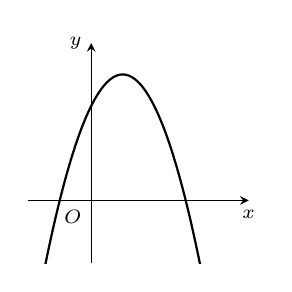
\begin{tikzpicture}[>=stealth,x=1cm,y=1cm,scale=0.4]
			\def\a{-1} % Hệ số a phải khác 0
			\def\b{2}
			\def\c{3}
			%\draw[color=gray,dash pattern=on 1pt off 1pt,xstep=1.0cm,ystep=1.0cm] (-2.2,-2.2) grid (5.2,5.2);
			\draw[->] (-2,0) -- (5,0) node[below] {\scriptsize $x$};
			\draw[->] (0,-2) -- (0,5) node[left] {\scriptsize $y$};
			\draw (0,0)node[below left]{\scriptsize $O$};
			\pgfmathsetmacro\xdinh{-(\b)/2*(\a)}
			\pgfmathsetmacro\ydinh{(4*(\a)*(\c)-(\b)^2)/(4*(\a))}
			%\fill[dashed] (\xdinh,\ydinh)circle(2pt) edge (\xdinh,0) edge (0,\ydinh);
			\clip (-2,-2)rectangle(5,5);
			\draw[thick,samples=150,smooth,domain=-5:5] plot(\x,{\a*(\x)^2+(\b)*\x+(\c)});
		\end{tikzpicture}
	}
	\loigiai{
		\begin{itemchoice}
	\itemch Dựa vào đồ thị hàm số ta thấy hàm số đồng biến trên $(-\infty;0)$.
	\itemch Đồ thị hàm số cắt trục hoành tại hai điểm phân biệt có hoành độ trái dấu.
	\itemch Đồ thị cắt trục tung tại điểm $(0;c)$ có tung độ dương nên $c>0$
	\itemch Đồ thị có bề lõm hướng xuống nên $a<0$.\\
	Đồ thị có hoành độ đỉnh dương nên $-\dfrac{b}{2a}>0 \Leftrightarrow \dfrac{b}{a}<0 $ và do $a<0$ nên $b>0$.
	\end{itemchoice}
	}
\end{ex}
\begin{ex}%[0H5V3-3]	
Cho tam giác $ABC$. Gọi $M$, $G$ lần lượt là trung điểm $BC$ và trọng tâm tam giác $ABC$. Khi đó
\choiceTF
{\True $2\overrightarrow{GM}+\overrightarrow{GA}=\vec{0}$}
{\True $\overrightarrow{MA}+\overrightarrow{MB}+\overrightarrow{MC}=3\overrightarrow{MG}$}
{\True $\overrightarrow{BA}+\overrightarrow{BC}=3\overrightarrow{BG}$}
{Nếu điểm $P$ thỏa mãn $3\overrightarrow{PA}+\overrightarrow{PB}+\overrightarrow{PC}=3\overrightarrow{MG}$ thì $P$ là trung điểm $AG$}
\loigiai{
\immini{
\begin{itemchoice}
\itemch	Ta có $GA=2GM$ nên $2\overrightarrow{GM}+\overrightarrow{GA}=\vec{0}$
\itemch Ta có $\overrightarrow{MA}+\overrightarrow{MB}+\overrightarrow{MC}=\overrightarrow{MA}=3\overrightarrow{MG}$
\itemch $\overrightarrow{BA}+\overrightarrow{BC}=\overrightarrow{GA}-\overrightarrow{GB}+\overrightarrow{GC}-\overrightarrow{GB}=(\overrightarrow{GA}+\overrightarrow{GB}+\overrightarrow{GC})-3\overrightarrow{GB}=3\overrightarrow{BG}$
\itemch Ta có $3\overrightarrow{PA}+\overrightarrow{PB}+\overrightarrow{PC}=3\overrightarrow{MG}\Leftrightarrow 5\overrightarrow{PG}+3\overrightarrow{GA}+\overrightarrow{GB}+\overrightarrow{GC}=3\overrightarrow{MG}\Leftrightarrow 5\overrightarrow{PG}+\dfrac{1}{2}\overrightarrow{GA}=\vec{0}\Leftrightarrow \overrightarrow{GA}=10\overrightarrow{GP}$
\end{itemchoice}
}{
\begin{tikzpicture}[>=stealth,x=1cm,y=1cm,line width=1pt, scale=1]
	\coordinate[label = left:$A$] (A) at (0,0);
	\coordinate[label = left:$B$] (B) at (2.5,4);
	\coordinate[label = right:$C$] (C) at (6,-0.5);
	\coordinate[label = right:$M$] (M) at ($(B)!1/2!(C)$);
	\coordinate[label = above:$G$] (G) at ($(A)!2/3!(M)$);
	\coordinate[label = below:$P$] (P) at ($(G)!1/10!(A)$);
	\draw (A)--(B)--(C)--(A)--(M);
	\foreach \x in {A,B,C,M,G,P} \fill[black] (\x) circle (1.5pt);
\end{tikzpicture}
}
}
\end{ex}
\begin{ex}%[0D6H4-4]
	Bảng dưới đây thống kê tổng số giờ nắng trong năm $2019$ theo từng tháng được đo bởi hai trạm quan sát khí tượng đặt ở Tuyên Quang và Cà Mau.
	\begin{center} 
		\begin{tabular}{|c|c|c|c|c|c|c|c|c|c|c|c|c|} 
			\hline 
			\textbf{Tháng} & $ 1$ & $2$ & $3$ & $4$ & $5$ & $6$ & $7$ & $8$ & $9$ & $10$ & $11$ & $12$\\ 
			\hline 
			\textbf{Tuyên Quang} & $25$ & $89$ & $72$ & $117$ & $106$ & $177$ & $156$ & $203$ & $227$ & $146$ & $117$ & $145$\\ 
			\hline 
			\textbf{Cà Mau} & $180$ & $223$ & $257$ & $245$ & $191$ & $111$ & $141$ & $134$ & $130$ & $122$ & $157$ & $173$\\ 
			\hline 
		\end{tabular}
	\end{center}
	\choiceTF
	{\True Số trung bình tổng số giờ nắng của Tuyên Quang là $131{,}6$ giờ }
	{Phương sai của tổng số giờ nắng của Tuyên Quang là $3\,681,79$}
	{\True Độ lệch chuẩn của tổng số giờ nắng của Cà Mau là $48,8$}
	{\True Tổng số giờ nắng mỗi tháng ờ Tuyên Quang thay đổi nhiều hơn ở Cà Mau}
	\loigiai{
		
	\begin{itemchoice}
	\itemch Số trung bình tổng số giờ nắng của Tuyên Quang\\
		$ \dfrac{\left(25+89+72+117+106+177+156+203+227+146+117+145\right)}{12}=\dfrac{395}{3}\approx132.$
	\itemch	Phương sai\\ 
		$\dfrac{1}{12}\left(25^2+89^2+72^2+117^2+106^2+177^2+156^2+203^2+227^2+146^2\right.$\\ $\left.+117^2+145^2\right)-\left(\dfrac{395}{3}\right)^2\approx 3\,186,79$\\
		Độ lệch chuẩn $\approx 56,45$.
	\itemch	Số trung bình tổng số giờ nắng của Cà Mau\\
		$\dfrac{1}{12}\left(180+223+257+245+191+111+141+134+130+122+157+173\right)=172$
		Phương sai \\
		$\dfrac{1}{12}\left(180^2+223^2+257^2+245^2+191^2+111^2+141^2+134^2+130^2+122^2\right.$\\ $\left.+157^2+173^2\right)\approx 2\,381,45$\\
		Độ lệch chuẩn $\approx 48,8$.
	\itemch Tổng số giờ nắng mỗi tháng ờ Tuyên Quang thay đổi nhiều hơn ở Cà Mau.
	\end{itemchoice}
	}
\end{ex}
\begin{ex}%[0D6H3-3]
Trong một cuộc thi nghề, người ta ghi lại thời gian (đơn vị: phút) hoàn thành một sản phẩm của một số thí sinh ở bảng sau
\begin{center}\begin{tabular}{|c|l|l|l|l|l|}
	\hline Thời gian & $5$ & $6$ & $7$ & $8$ & $9$ \\
	\hline Số thí sinh & $1$ & $3$ & $5$ & $2$ & $1$ \\
	\hline
\end{tabular}\end{center}
\choiceTF
{\True Số trung bình của mẫu số liệu $\overline{x}=6{,}9$}
{\True Trung vị của mẫu số liệu $Q_2=7$}
{Khoảng tứ phân vị $\Delta Q=0{,}5$}
{\True Mốt của mẫu số liệu $M_{\text{o}}=7$}
\loigiai{
\begin{itemchoice}
\itemch Số trung bình $\bar{x}=\dfrac{5 \cdot 1+6 \cdot 3+7 \cdot 5+8 \cdot 2+9 \cdot 1}{12}=6{,}9$
\itemch	Sắp xếp mẫu số liệu theo thứ tự không giảm
		$$\begin{array}{llllllllllll}5 & 6 & 6 & 6 & 7 & 7 & 7 & 7 & 7 & 8 & 8 & 9\end{array}$$
		Cỡ mẫu là $12$ (chẵn)\\
		Số trung vị $M_e=\dfrac{x_6+x_7}{2}=\dfrac{7+7}{2}=7$.
\itemch Ta có 
\begin{itemize}
\item Tứ phân vị thứ nhất: $Q_1=\dfrac{x_3+x_4}{2}=\dfrac{6+6}{2}=6$.
\item Tứ phân vị thứ hai: $Q_2=\dfrac{x_6+x_7}{2}=\dfrac{7+7}{2}=7$.	
\item Tứ phân vị thứ ba: $Q_3=\dfrac{x_9+x_10}{2}=\dfrac{7+8}{2}=7{,}5$.
\item Khoảng tứ phân vị là $\Delta Q=Q_3-Q_1=1{,}5$.
\end{itemize}
\itemch	Dễ thấy Mốt $M_0=7$.
\end{itemchoice}}
\end{ex}
\Closesolutionfile{ans}
\indapan{3}{ans/ans-1-OTHK1-De3-DS}
%-------------------------------------------
\Opensolutionfile{ans}[ans/ans-1-OTHK1-De3-KQ]
\caukq
\begin{ex}%[0D6H4-4]
Kết quả điểm thi học kì $1$ của một học sinh lớp $10$ như sau
\begin{center}\begin{tabular}{|l|l|l|l|l|l|l|l|l|}
	\hline $4$ & $9$ &$5$ & $8$ & $10$ & $7$ & $6$ & $5$ & $8$ \\
	\hline
\end{tabular}\end{center}
Phương sai của mẫu số liệu trên là (làm tròn đến hàng phần trăm).
\shortans[3]{$3{,}64$}
	\loigiai{
		Sắp xếp lại dãy số theo thứ tự không giảm$\colon 4;\quad 5;\quad 5;\quad 6;\quad 7;\quad 8;\quad 8;\quad 9;\quad 10$.\\
		Số trung bình cộng $\overline{x}=\dfrac{4+5\cdot 2+6+7+8\cdot 2+9+10}{9}=6{,}89$.\\
		Phương sai $s^2=\dfrac{1}{9}(4^2+2\cdot 5^2+6^2+7^2+2\cdot 8^2+9+10)-6{,}89^2=3{,}64$.
	}
\end{ex}
\begin{ex}%[0D6H3-3]
	Số bàn thắng mà một đội bóng ghi được ở mỗi trận đấu trong một mùa giải được thống kê lại ở bảng sau:
	\begin{center}
		\begin{tabular}{|c|c|c|c|c|c|c|}
			\hline Số bàn thắng & $0$ & $1$ & $2$ & $3$ & $4$ & $6$ \\
			\hline Só trận & $5$ & $10$ & $5$ & $3$ & $2$ & $1$ \\
			\hline
		\end{tabular}
	\end{center}
	Hãy xác định số bàn thắng trung bình đội đó ghi được trong một trận đầu của mùa giải.
\shortans[3]{$1{,}65$}
	\loigiai{
		Bảng số liệu trên được cho dưới dạng bảng tần số.\\	
		Số trận đấu trong toàn mùa giải hay chính là cỡ mẫu là
		$n = 5 + 10 + 5 + 3 + 2 + 1 = 26$ (trận).\\	
		Số bàn thắng trung bình của đội đó ghi được trong một trận đấu của mùa giải là	
		$$\bar{x}=\frac{5\cdot 0+10\cdot 1+5\cdot 2+3\cdot 3+2\cdot 4+1\cdot 6}{26}\approx 1{,}65.$$
		
	}
\end{ex}
\begin{ex}%[0D3H2-6]
	Người ta đóng $4$ cái cột xuống đất thành hình chữ nhật sao cho có thể dùng đủ $10$ m dây (không co dãn) để cột xung quanh. Khi hình chữ nhật có diện tích lớn nhất thì độ dài đường chéo của nó bằng.
\shortans[3]{$3{,}54$}
	\loigiai{
		Gọi $x$, $5-x$ là các kích thước của hình chữ nhật.\\
		Diện tích hình chữ nhật $S(x)=x\left(5-x \right)=-x^2+5x$.\\
		$S(x)$ là hàm số bậc hai có đồ thị là một Parabol có $a=-1<0$.\\
		$S(x)$ đạt giá trị lớn nhất $\Leftrightarrow x=\dfrac{-b}{2 a}=2,5$ (m).\\
		Vậy hình chữ nhật có diện tích lớn nhất là hình vuông cạnh $2{,}5$ m. Khi đó độ dài đường chéo bằng $l=3{,}54$ cm
	}
\end{ex}
\begin{ex}%[0H4V3-2]
Trong chuyến tham quan hoạt động ngoại khoá tại Đà Lạt của trường THPT A, hai bạn Bình và An cùng thực hiện một ý định rất thú vị đó là đo chiều cao của \lq\lq \textit{Khối nụ hoa Atisô} \rq\rq \, ở Quảng trường Lâm Viên. Hai bạn đã thực hiện các phép đo đạc được mô hình hóa lại như sau: An đứng ở vị trí $A$, Bình đứng ở vị trí $B$, chân nụ hoa ở vị trí $C$, đỉnh nụ hoa ở vị trí $D$. Biết rằng ba điểm $A$, $B$, $C$ thẳng hàng và cạnh $CD$ vuông góc với cạnh $AC$. Cho biết các số đo $AB=3{,}5$ mét, $\widehat{BA D}=55^{\circ}$, $\widehat{CB D}=65^{\circ}$. Em hãy giúp hai bạn tính chiều cao của \lq\lq \textit{Khối nụ hoa Atisô}\rq\rq \, với những đo đạc trên? (làm tròn đến hàng phần chục).

{\centering
\includegraphics[scale=.4]{images/Nuhoa.jpg}
\begin{tikzpicture}[scale=0.8, font=\footnotesize, line join=round, line cap=round,line width=1pt, >=stealth]	
		\coordinate[label=below:$C$](C) at (-5,0.8); 
		\coordinate[label=above:$D$](D) at (-5,7.7); 
		\coordinate[label=below:$B$](B) at (1.2,0.8); 
		\coordinate[label=below right:$A$](A) at (3,0.8); 
		\draw (D)--(C)--(B)--cycle	(D)--(A);
		\draw pic[draw,angle radius=4mm]{right angle=D--C--A};
		\draw pic[draw,blue,angle radius=4mm,angle eccentricity=1.5,"$65^{\circ}$"] {angle = D--B--C}; 
		\draw pic[draw,blue,angle radius=4mm,angle eccentricity=1.5,"$55^{\circ}$"] {angle = D--A--C}; 
		\draw 	(B)--(A) node[pos=0.5,sloped,below]{$3{,}5\text{m}$};
		\end{tikzpicture}}
	\shortans[3]{$15$}
	\loigiai{
		\immini{ Ta có $\widehat{AD B}=180^{\circ}-\widehat{AB D}-\widehat{DA B}=10^{\circ}$.\\
			Áp dụng định lí sin trong tam giác $ABD$ ta có
			$$
			\dfrac{AB}{\sin 10^{\circ}}=\dfrac{BD}{\sin 55^{\circ}} \Rightarrow BD=\dfrac{3{,}5 \cdot \sin 55^{\circ}}{\sin 10^{\circ}}
			$$
			Trong tam giác $BCD$
			$$
			CD=BD \cdot \sin 65^{\circ}=\dfrac{3{,}5 \cdot \sin 55^{\circ}}{\sin 10^{\circ}} \cdot \sin 65^{\circ} \approx 15{,}0 \text { (mét)}
			$$
			Vậy chiều cao của \lq\lq \textit{Khối nụ hoa Atisô}\rq\rq \, xấp xỉ $15,0$ (mét)}
		{\begin{tikzpicture}[scale=.9, font=\footnotesize, line join=round, line cap=round, >=stealth]
				\coordinate[label=below:$C$](C) at (0,0); 
				\coordinate[label=above:$D$](D) at (0,7); 
				\coordinate[label=below:$B$](B) at (3,0); 
				\coordinate[label=below right:$A$](A) at (5,0); 
				\draw (D)--(C)--(B)--cycle	(D)--(A);
				\draw pic[draw,angle radius=4mm]{right angle=D--C--A};
				\draw pic[draw,blue,angle radius=4mm,angle eccentricity=1.5,"$65^{\circ}$"] {angle = D--B--C}; 
				\draw pic[draw,blue,angle radius=4mm,angle eccentricity=1.5,"$55^{\circ}$"] {angle = D--A--C}; 
				\draw 	(B)--(A) node[pos=0.5,sloped,below]{$3{,}5\text{m}$}; %Tùy chọn sloped,above,below
			\end{tikzpicture}
		}
	}
\end{ex}
\begin{ex}%[0H5V2-1]
	\immini{Phân tử sulfur dioxide (SO$_2$) có cấu tạo hình chữ V, góc liên kết $\widehat{OSO}$ gần bằng $120^\circ$. Người ta biểu diễn sự phân cực giữa nguyên tử S với mỗi nguyên tử O bằng các véc-tơ $\vec{\mu}_1$ và $\vec{\mu}_2$ có cùng phương với liên kết cộng hóa trị, có chiều từ nguyên tử S về mỗi nguyên tử O và cùng có độ dài là $1{,}6$ đơn vị (hình bên). Cho biết véc-tơ tổng $\vec{\mu}=\vec{\mu}_1+\vec{\mu}_2$ được dùng để biểu diễn sự phân cực của cả phân tử SO$_2$. Tính độ dài của $\vec{\mu}$.
	}{
		\begin{tikzpicture}[scale=1, font=\footnotesize, line join=round, line cap=round, >=stealth]
			\path 
			(0,0) coordinate (S)
			(S)+(-150:3) coordinate (O1) node[above]{$O$}
			(S)+(-30:3) coordinate (O) node[above]{$O$}
			($(O)+(O1)-(S)$) coordinate (m)
			;
			\draw (S) circle (.45cm);
			\draw (O) circle (.45cm) (O1) circle (.45cm);
			\draw[->] (S)--(O) node[above,sloped,pos=.5] {$\vec{\mu}_2$}; \draw[->] (S)--(O1) node[above,sloped,pos=.5] {$\vec{\mu}_1$}; \draw[->] (S)--(m) node[above,sloped,pos=.5] {$\vec{\mu}$};
			\draw[dashed] (O)--(m)--(O1);
			\foreach \p/\r in {S/90}
			\fill (\p) circle (1.5pt) node[shift={(\r:3mm)}]{$\p$};
		\end{tikzpicture}
	}
	\shortans[3]{$2{,}56$}
	\loigiai{
		Ta có $\vec{\mu}_1\cdot \vec{\mu}_2=\left|\vec{\mu}_1\right|\cdot \left|\vec{\mu}_2\right|\cdot \cos \left(\vec{\mu}_1,\vec{\mu}_2\right)=1{,}6\cdot 1{,}6\cdot \cos 120^\circ=-1{,}28$.\\
		Khi đó
		\begin{eqnarray*}
			|\vec{\mu}|^2&=&\vec{\mu}^2=\left(\vec{\mu}_1+\vec{\mu}_2\right)^2\\
			&=&\vec{\mu}_1^2+2\cdot \vec{\mu}_1\cdot \vec{\mu}_2+\vec{\mu}_2^2\\
			&=&\left|\vec{\mu}_1\right|^2+2\cdot \vec{\mu}_1\cdot \vec{\mu}_2+\left|\vec{\mu}_2\right|^2\\
			&=&1{,}6^2+2\cdot -1{,}28+1{,}6^2=2{,}56.
		\end{eqnarray*}
	}
\end{ex}
	\begin{ex}%[0H5H2-1]

		Một máy bay có véc-tơ vận tốc chỉ theo hướng bắc, vận tốc gió là một véc-tơ theo hướng đông như hình bên. Tính độ dài véc-tơ tổng của hai véc-tơ nói trên.
		
	\begin{center}
		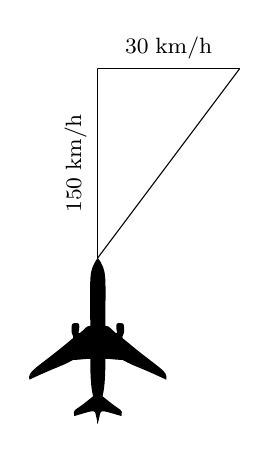
\begin{tikzpicture}[scale=0.6, font=\footnotesize, line join=round, line cap=round, >=stealth]
			\fill[black] (0,0)..controls +(-55:0.35) and +(90:1.1)..(0.16,-1.44)..controls +(0:0.1) and +(145:0.15)..(0.39,-1.6)..controls +(-20:0.03) and +(-40:0.02)..(0.4,-1.54)..controls +(110:0.03) and +(-120:0.02)..(0.4,-1.4)..controls +(70:0.03) and +(100:0.02)..(0.54,-1.4)..controls +(-40:0.03) and +(40:0.03)..(0.54,-1.62)..controls +(-120:0.1) and +(140:0.02)..(0.56,-1.73)..controls +(-40:1) and +(80:0.2)..(1.45,-2.58)..controls +(155:0.8) and +(-28:0.4)..(0.52,-2.16)..controls +(180:0.2) and +(0:0.2)..(0.16,-2.14)..controls +(-90:0.3) and +(75.6:0.2)..(0.1,-2.93)..controls +(-40:0.6) and +(85.6:0.18)..(0.5,-3.35)..controls +(164:0.57) and +(72.6:0.32)..(0.,-3.5)--cycle;
			\fill[black,xscale=-1] (0,0)..controls +(-55:0.35) and +(90:1.1)..(0.16,-1.44)..controls +(0:0.1) and +(145:0.15)..(0.39,-1.6)..controls +(-20:0.03) and +(-40:0.02)..(0.4,-1.54)..controls +(110:0.03) and +(-120:0.02)..(0.4,-1.4)..controls +(70:0.03) and +(100:0.02)..(0.54,-1.4)..controls +(-40:0.03) and +(40:0.03)..(0.54,-1.62)..controls +(-120:0.1) and +(140:0.02)..(0.56,-1.73)..controls +(-40:1) and +(80:0.2)..(1.45,-2.58)..controls +(155:0.8) and +(-28:0.4)..(0.52,-2.16)..controls +(180:0.2) and +(0:0.2)..(0.16,-2.14)..controls +(-90:0.3) and +(75.6:0.2)..(0.1,-2.93)..controls +(-40:0.6) and +(85.6:0.18)..(0.5,-3.35)..controls +(164:0.57) and +(72.6:0.32)..(0.,-3.5)--cycle;
			\draw[black] (0,0)--(0.,-3.5);
			\draw(0,0)--(0,4);
			\draw(0,4)--(3,4);
			\draw(0,0)--(3,4);
			\node[rotate=90,yshift=8] at (0,2){$150\mathrm{\;km/h}$};
			\node[above] at (1.5,4){$30\mathrm{\;km/h}$};
	\end{tikzpicture}\end{center}
	
	\shortans[3]{$153$}	
		\loigiai{
			Gọi $\vec{v}$ là véc-tơ vận tốc của máy bay và $\vec{g}$ là véc-tơ vận tốc gió.\\
			Theo giả thiết, ta có: $\left|\vec{v}\right|=150\mathrm{\;km/h}$ và $\left|\vec{g}\right|=30\mathrm{\;km/h}$.\\
			Do giá của $\vec{v}$ và $\vec{g}$ vuông góc nhau nên $\left|\vec{v}+\vec{g}\right|$ là cạnh huyền của tam giác vuông có hai cạnh góc vuông là $150$ và $30$.\\
			Do đó $\left|\vec{v}+\vec{g}\right|=\sqrt{150^2+30^2}=30\sqrt{26}\approx 153\mathrm{\;km/h}$.
		}

\end{ex}
\Closesolutionfile{ans}
\indapan{6}{ans/ans-1-OTHK1-De3-KQ}


